%\section{Compute-driven, Flight-Efficiency Optimization: A Case Study}
 
\label{sec:energy-case-study}
\section{Case Studies}
\label{sec:case-study}


We show how our closed-loop simulation, along with our open-source benchmark suite, can enable (1) performance, (2) energy and (3) reliability studies, both at the architecture and the holistic system-level. MAVBench simulation setup allows for inspection of intra-system, as well as system and environment interactions. Studying the intra-system interactions opens new avenues for hardware and software co-design, which we demonstrate in the form of onboard/edge-only compute versus offloading the compute to the unconstrained cloud. Studying the system and environment interactions can unlock new opportunities for trade-offs in computational complexity for energy efficiency, which we demonstrate using software-guided, hardware-assisted OctoMap resolution optimizations.

\subsection{A Performance Case Study}


As opposed to the study in Section~\ref{sec:char} where we emulated a fully-on-edge drone (i.e., a drone which all of its computation is done on the drone itself), we examine a cloud/edge drone where the computation is distributed across the edge and the cloud. We compare a fully-on-edge drone equipped with a TX2 versus a fully-in-cloud drone with a powerful cloud support. The ``cloud'' computational horsepower is composed of an Intel i7 4740 @ 4GHz with 32 GB of RAM and a GeForce GTX 1080. For network connectivity we utilize a 1Gbp/s LAN, which mimics a future 5G network~\cite{agyapong2014design, gupta2015survey}.

\begin{figure}[b!]
\centering
    \begin{subfigure}{.608\columnwidth}
    \centering
    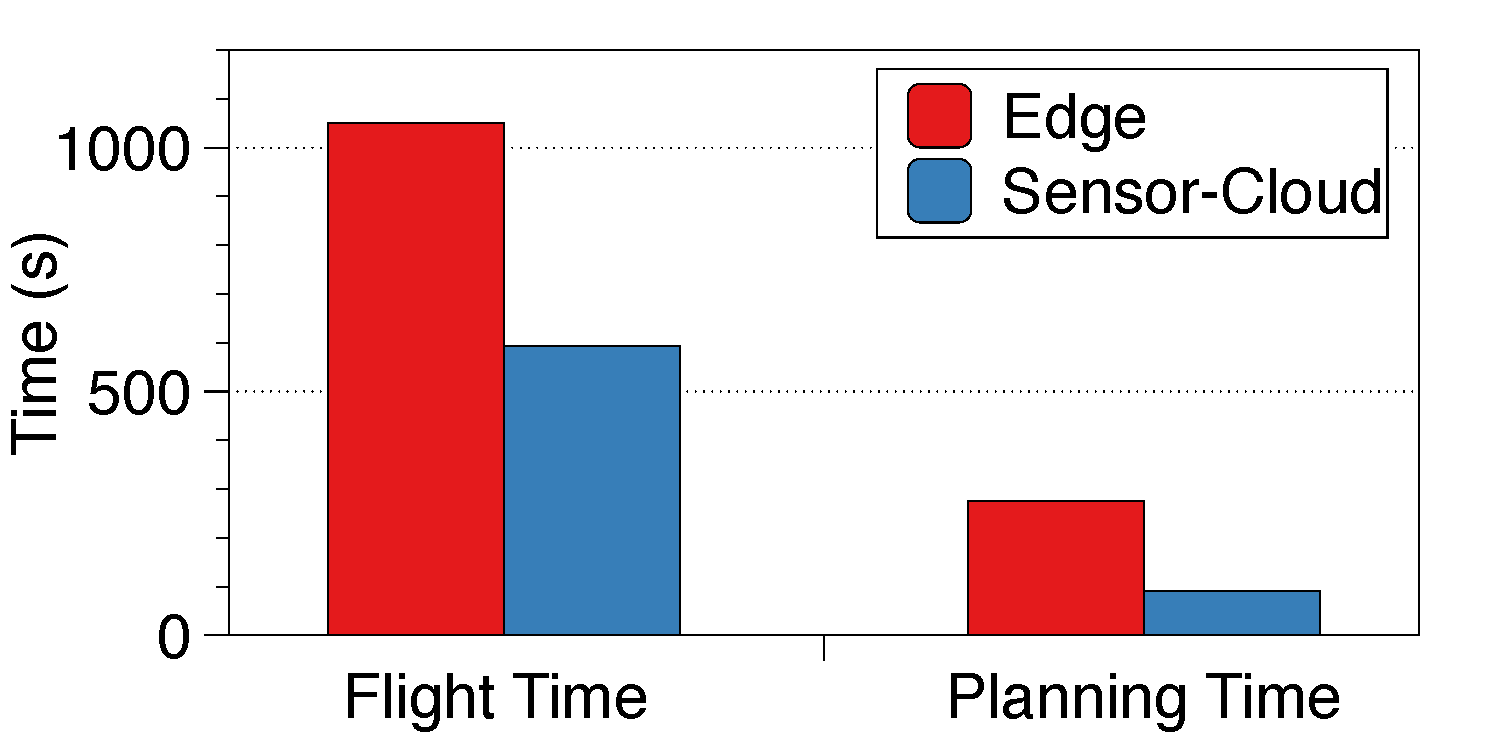
\includegraphics[trim=5 0 20 0, clip, width=\columnwidth]{figs/tx2-desktop_performance}
    \caption{Performance.}
    \label{Perforamnce}
    \end{subfigure}
    \hfill
    \begin{subfigure}{.365\columnwidth}
    \centering
    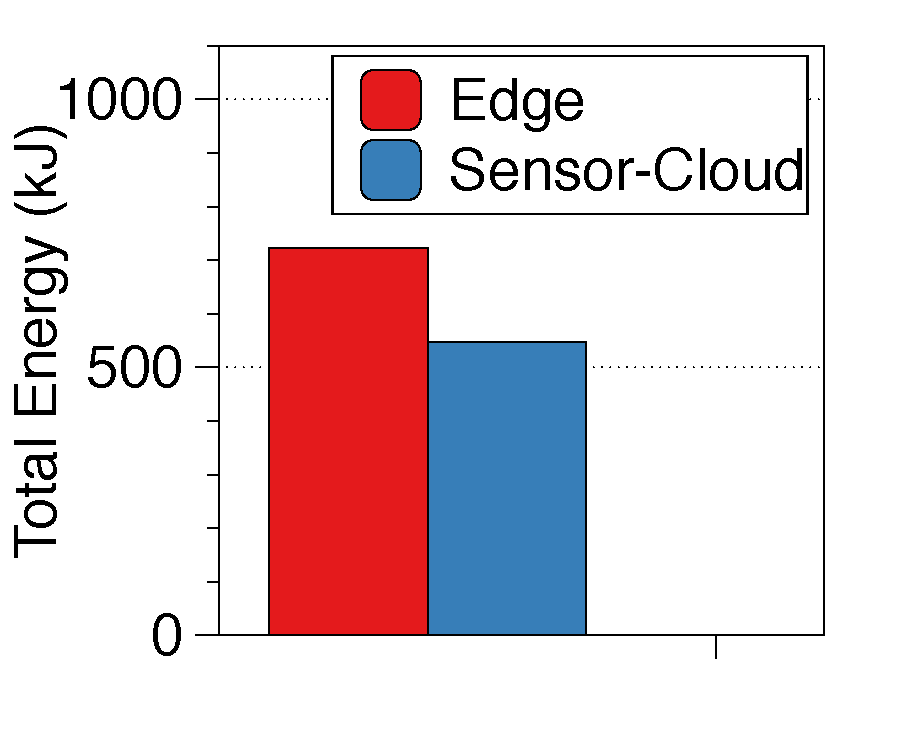
\includegraphics[trim=5 10 0 0, clip, width=\columnwidth]{figs/tx2-desktop_energy}
    \caption{Energy.}
    \label{fig:drone-power-time-series}
    \end{subfigure}
\caption{Comparing a full-on-edge drone versus a full-on-cloud drone. Our system allows part or portion of the MAVBench workloads to be offloaded to the cloud (or another local co-processing agent).}
\label{fig:cloud_edge}
\end{figure}

We target the planning stage of the PPC pipeline and focus on the 3D Mapping as the application of choice to offload. As we show in \Fig{fig:cloud_edge}, a drone that can enjoy the cloud's extra compute power sees a 3X speed up in planning time. This improves the drone's average velocity due to hover time reduction, and hence reduces the drone's overall mission time by as much as 50\%, effectively doubling its endurance.

\begin{figure*}[!t]
\vspace{-12pt}
    \centering
    \begin{subfigure}[t]{.24\linewidth}
        \centering
        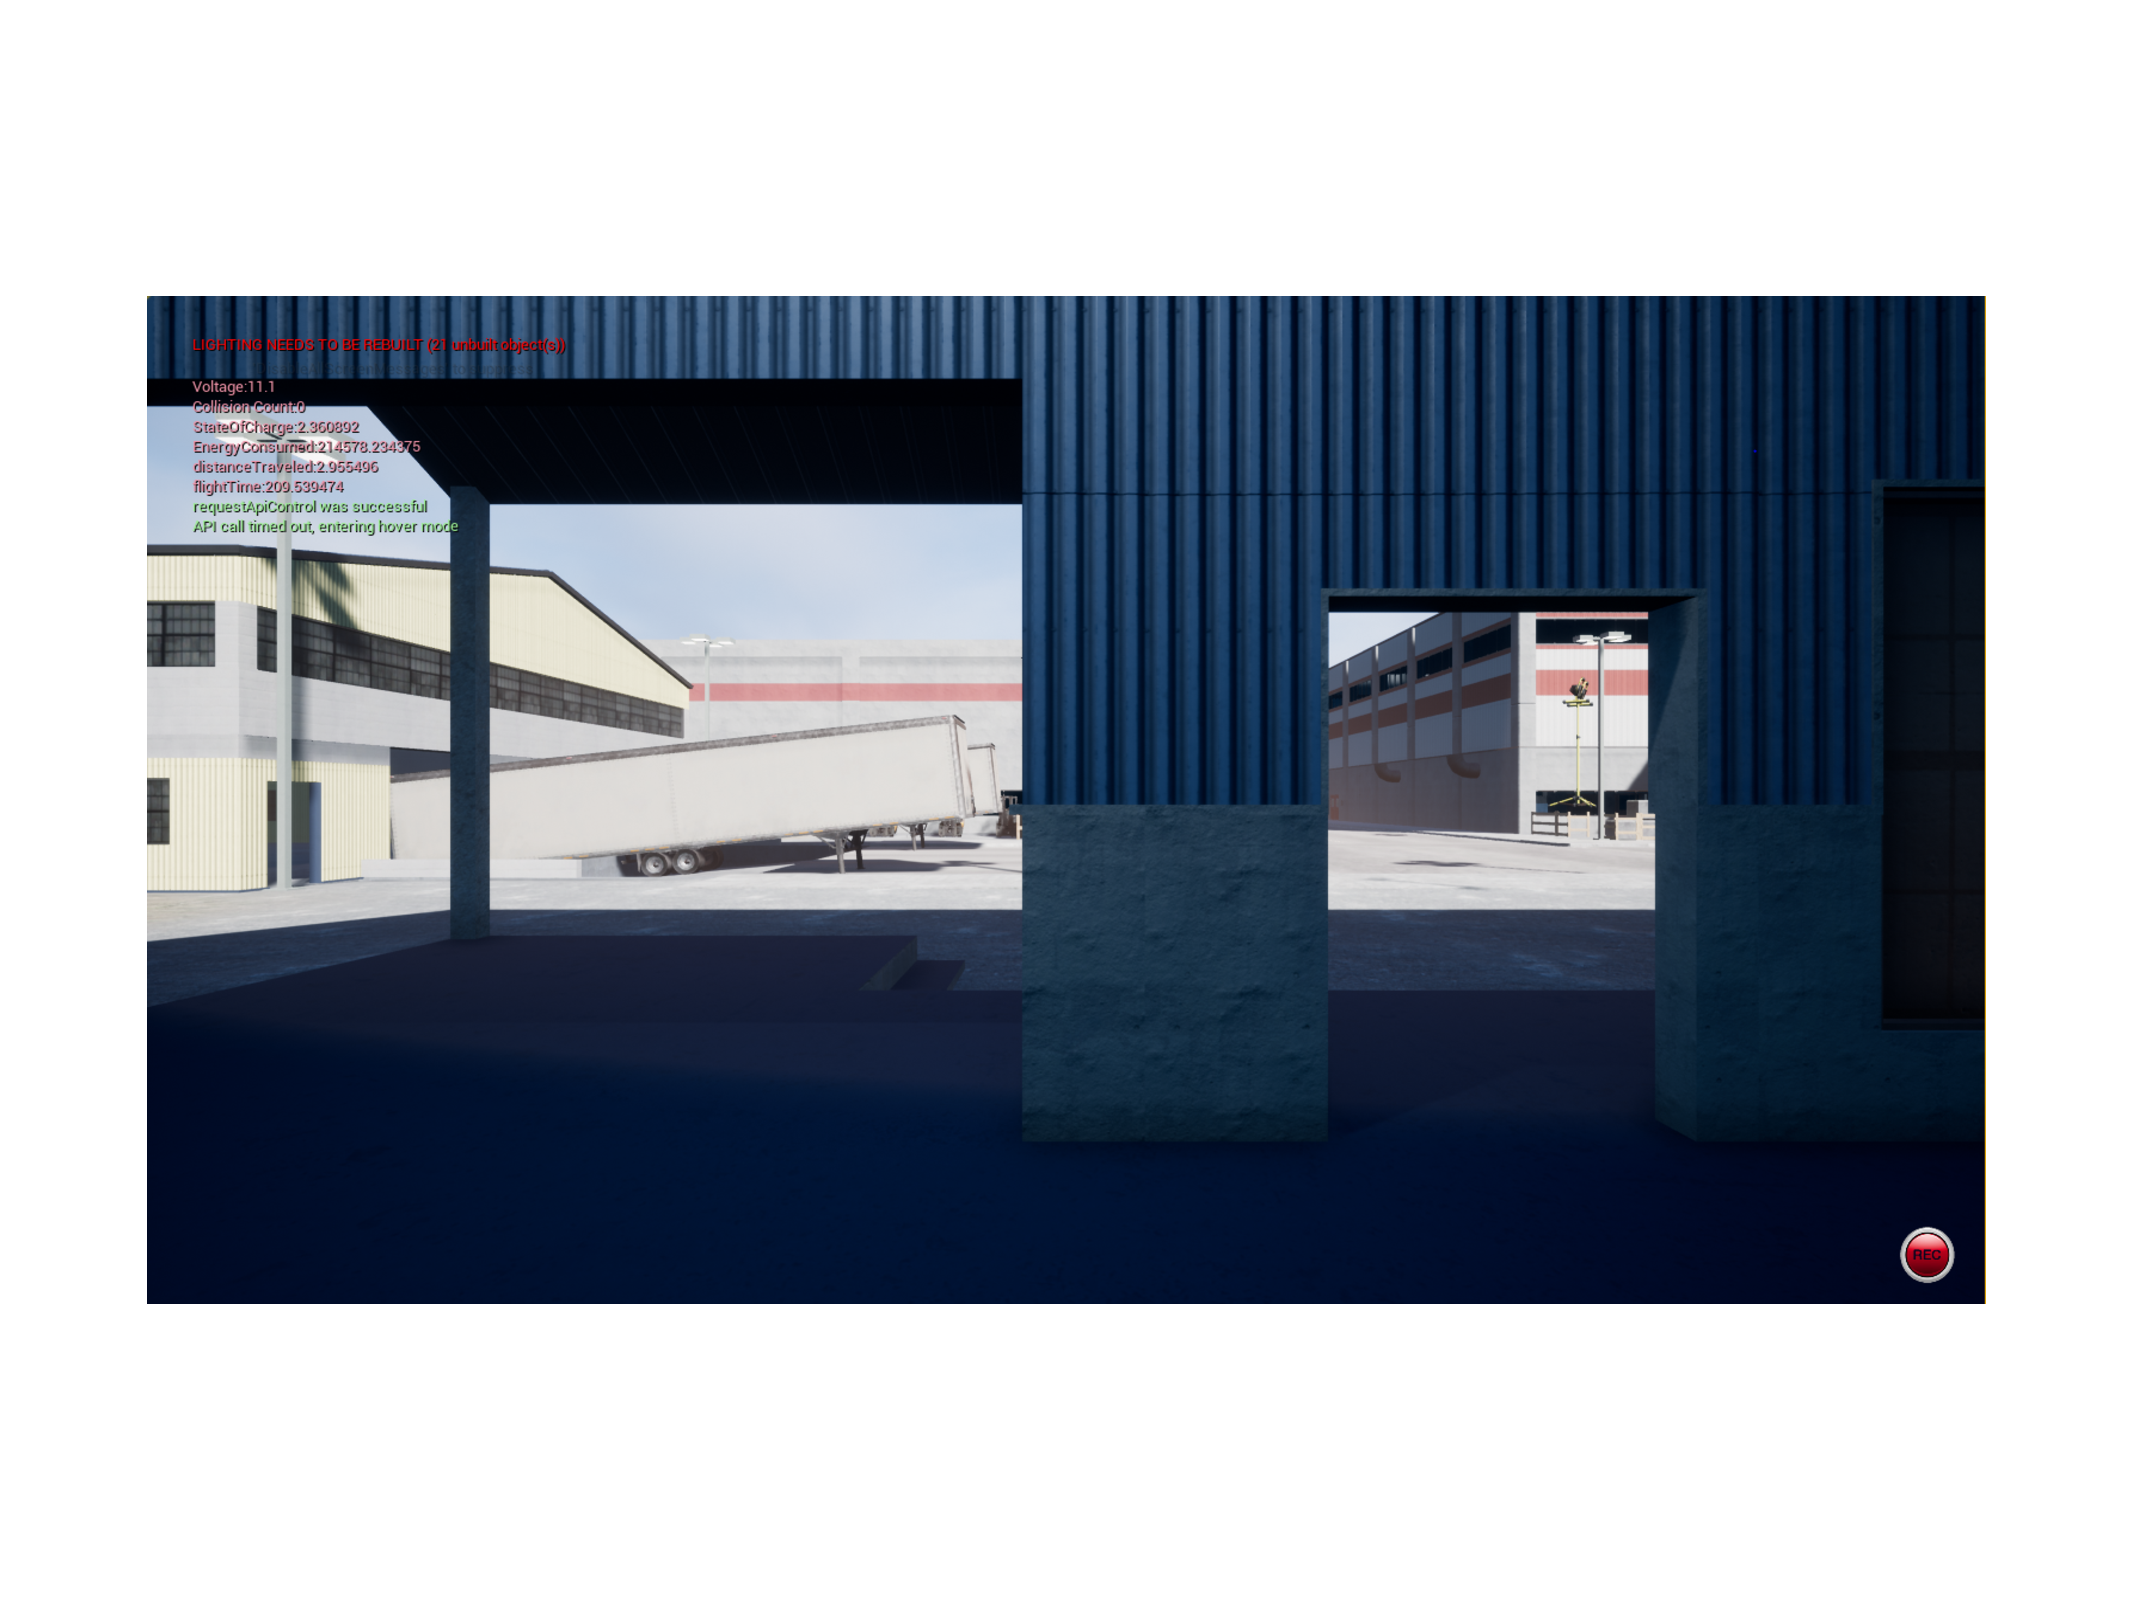
\includegraphics[height=1.4in]{figs/garage_sim}%
         \vspace{-20pt}
        \caption{Environment's map.}%
        \label{fig:garage_sim}
    \end{subfigure}
    \hfill
    \begin{subfigure}[t]{.24\linewidth}
        \centering
        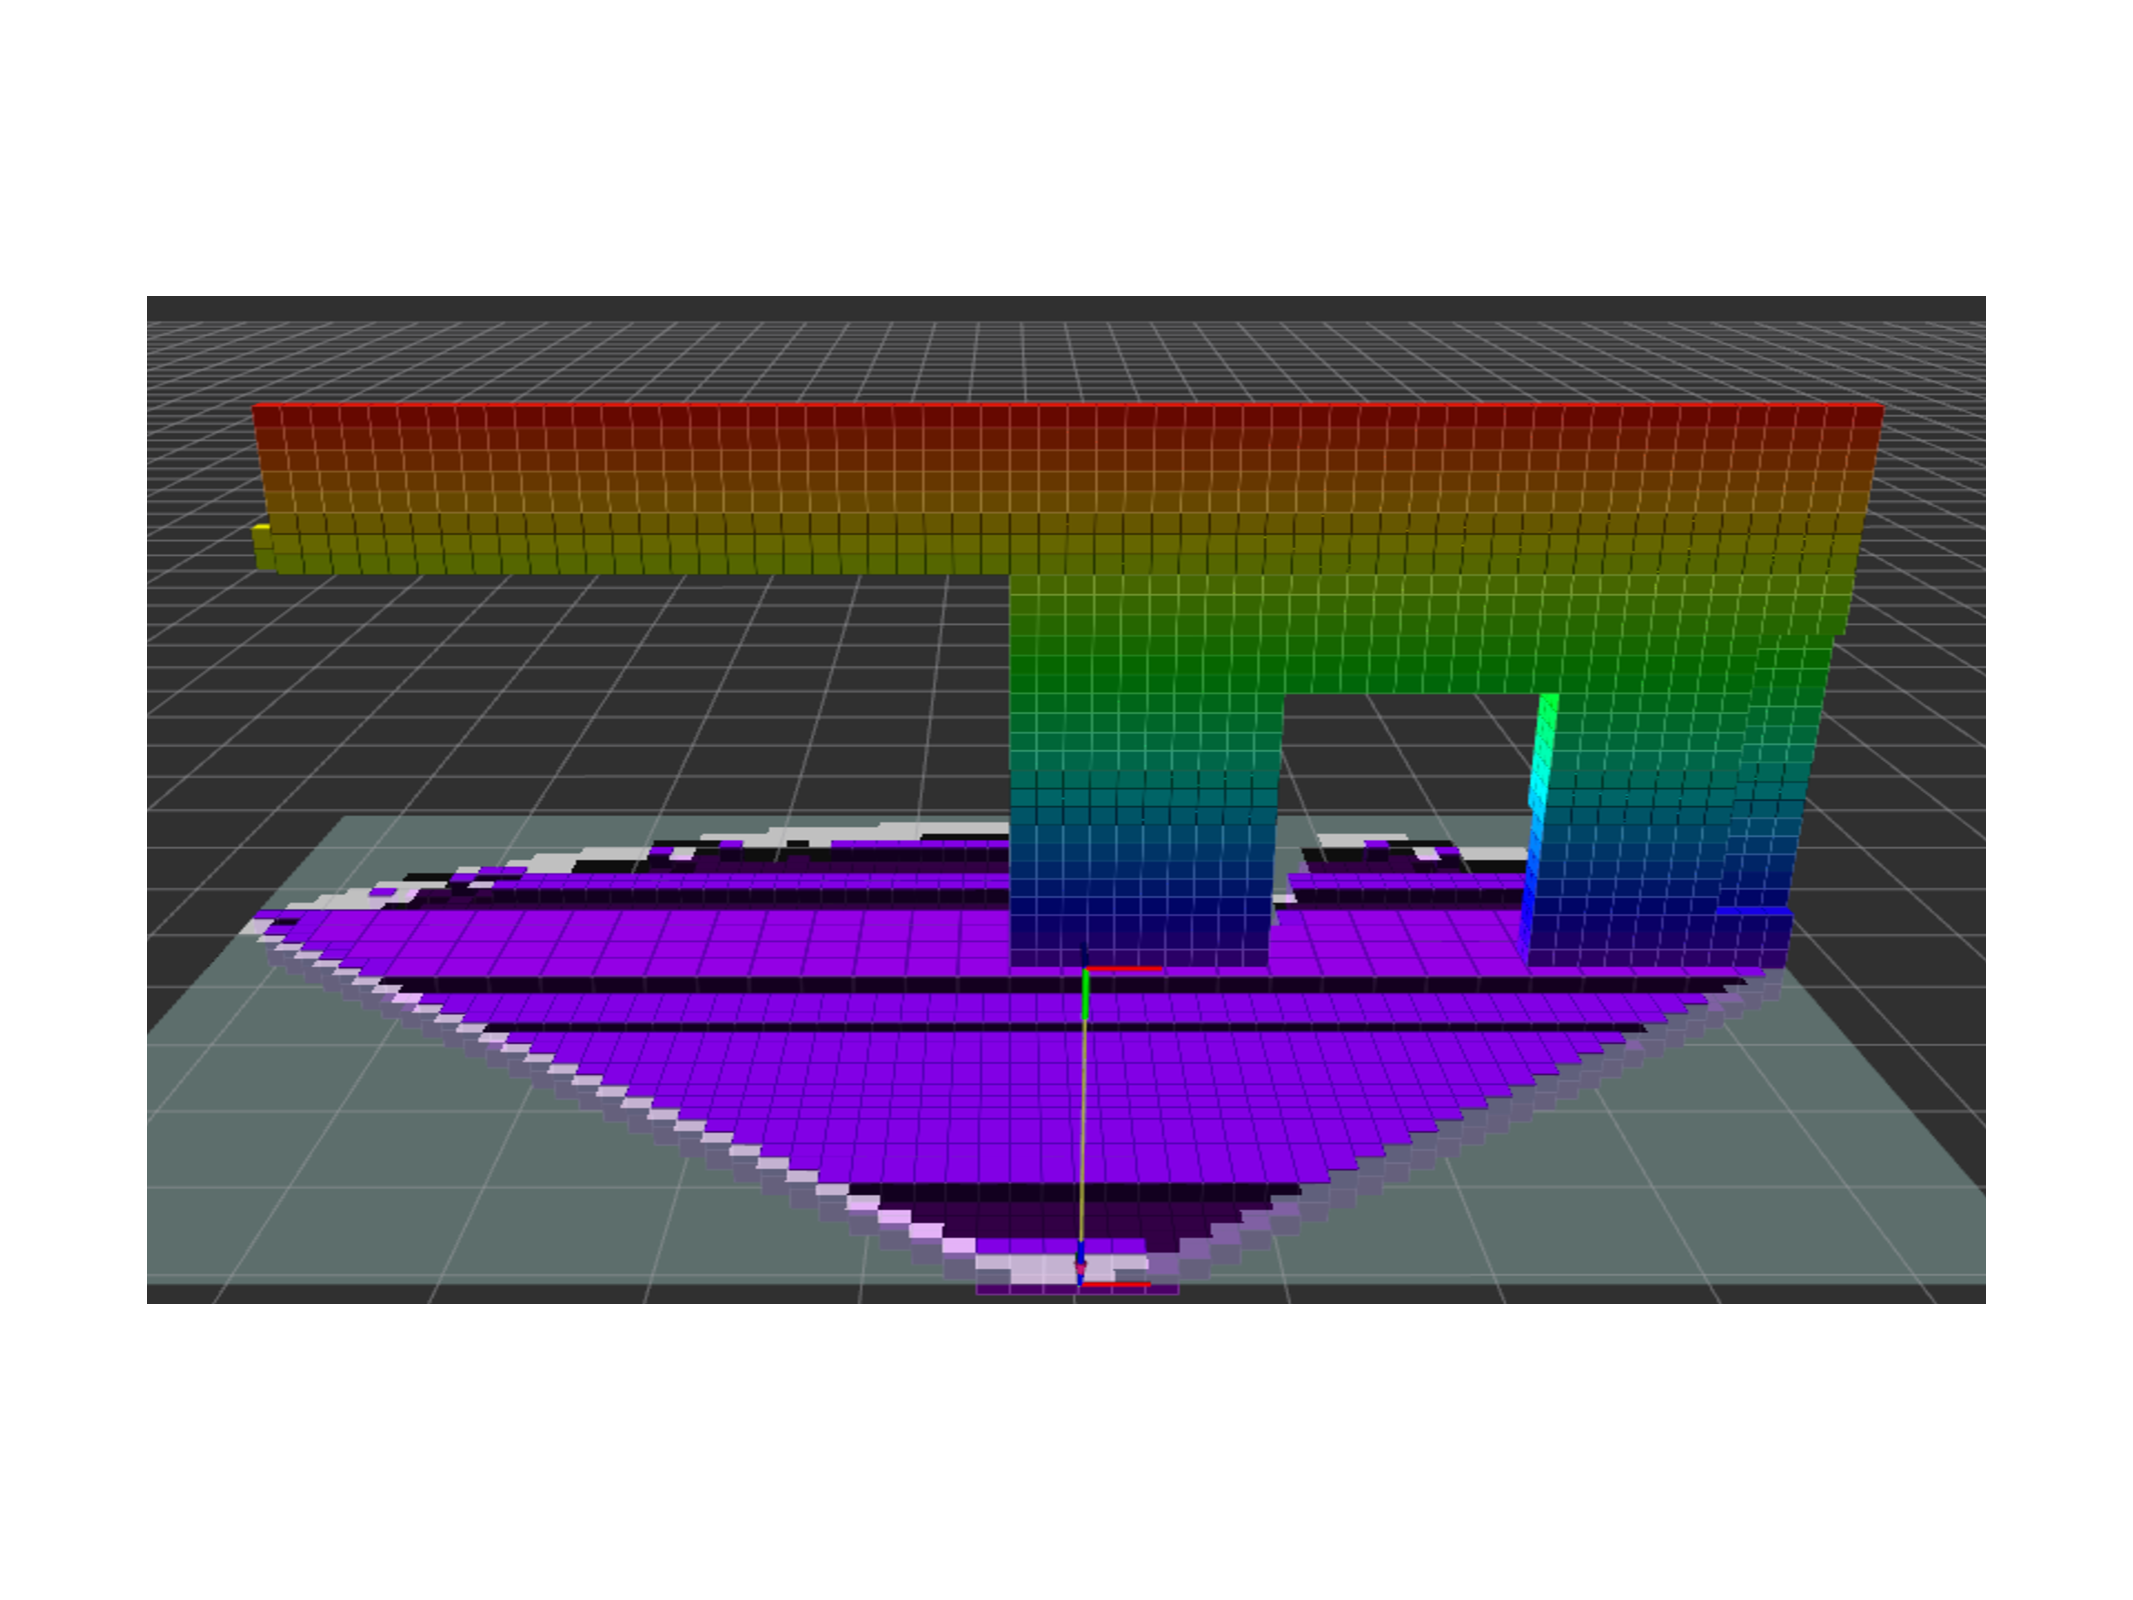
\includegraphics[height=1.4in]{figs/garage_rviz__15}%
         \vspace{-20pt}
        \caption{Resolution of 0.15 \emph{(m)}.}%
        \label{fig:rviz__15}
    \end{subfigure}
    \hfill
     \begin{subfigure}[t]{.24\linewidth}
        \centering
        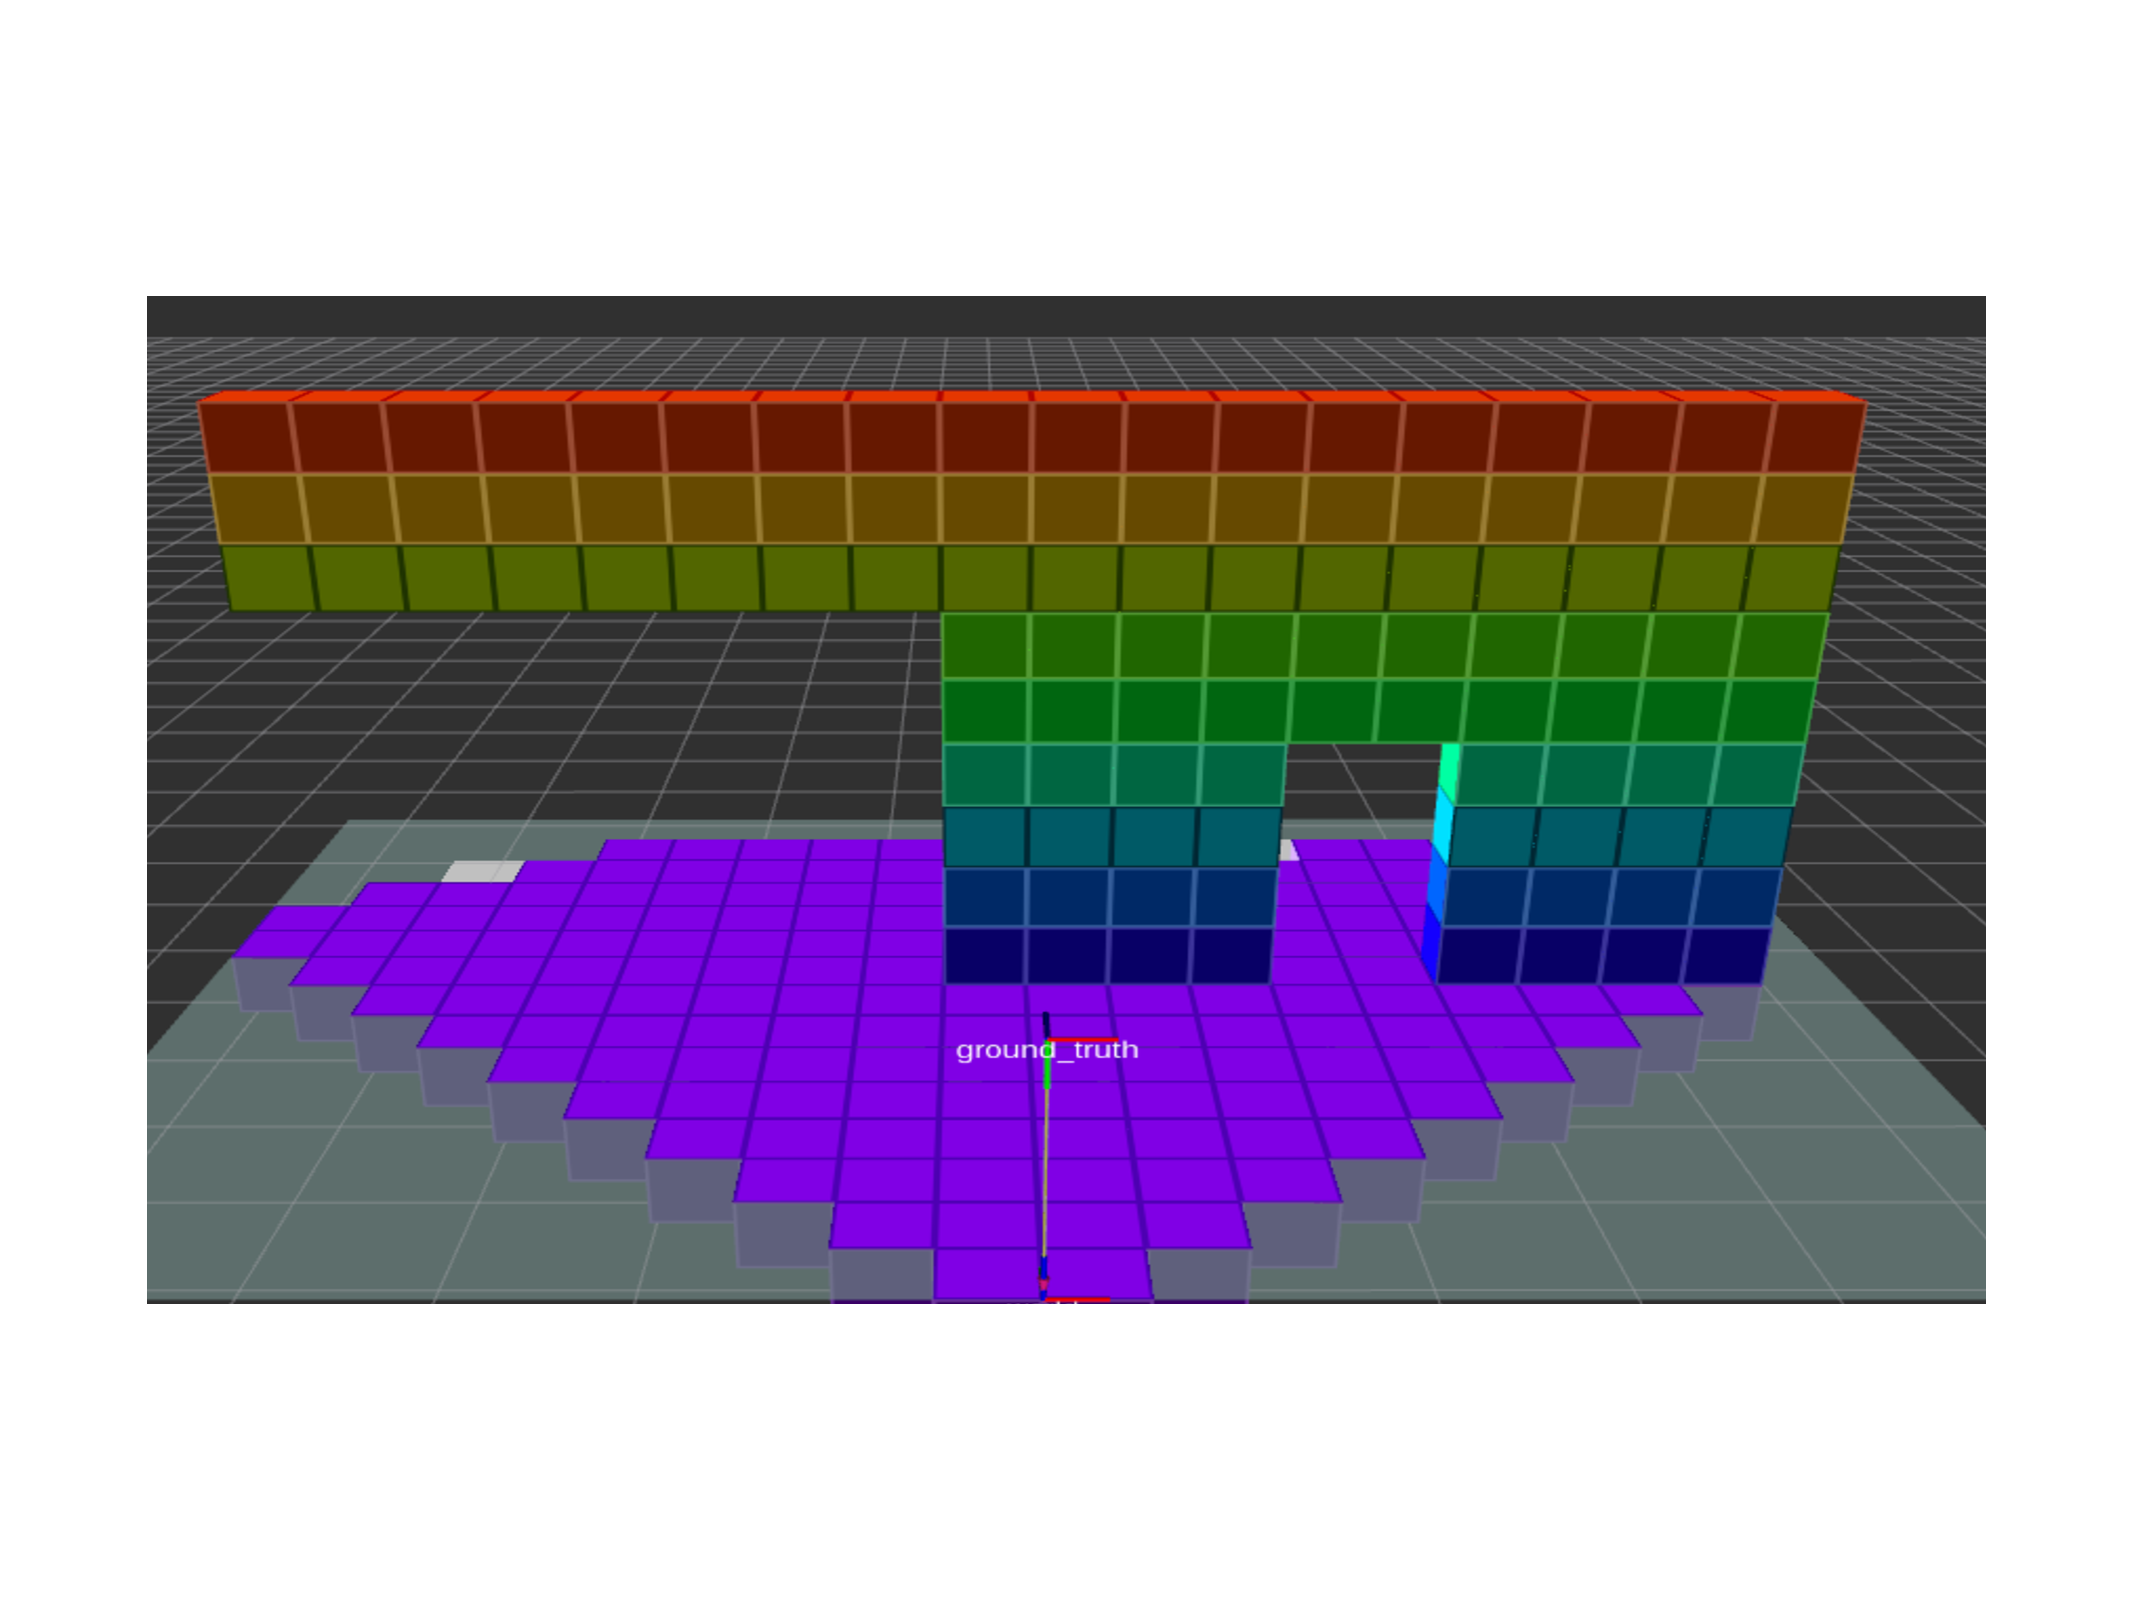
\includegraphics[height=1.4in]{figs/garage_rviz__5}%
      \vspace{-20pt}
     \caption{Resolution of 0.5 \emph{(m)}.}%
        \label{fig:game:rviz__5}
    \end{subfigure}
       \hfill
   \begin{subfigure}[t]{.24\linewidth}
        \centering
        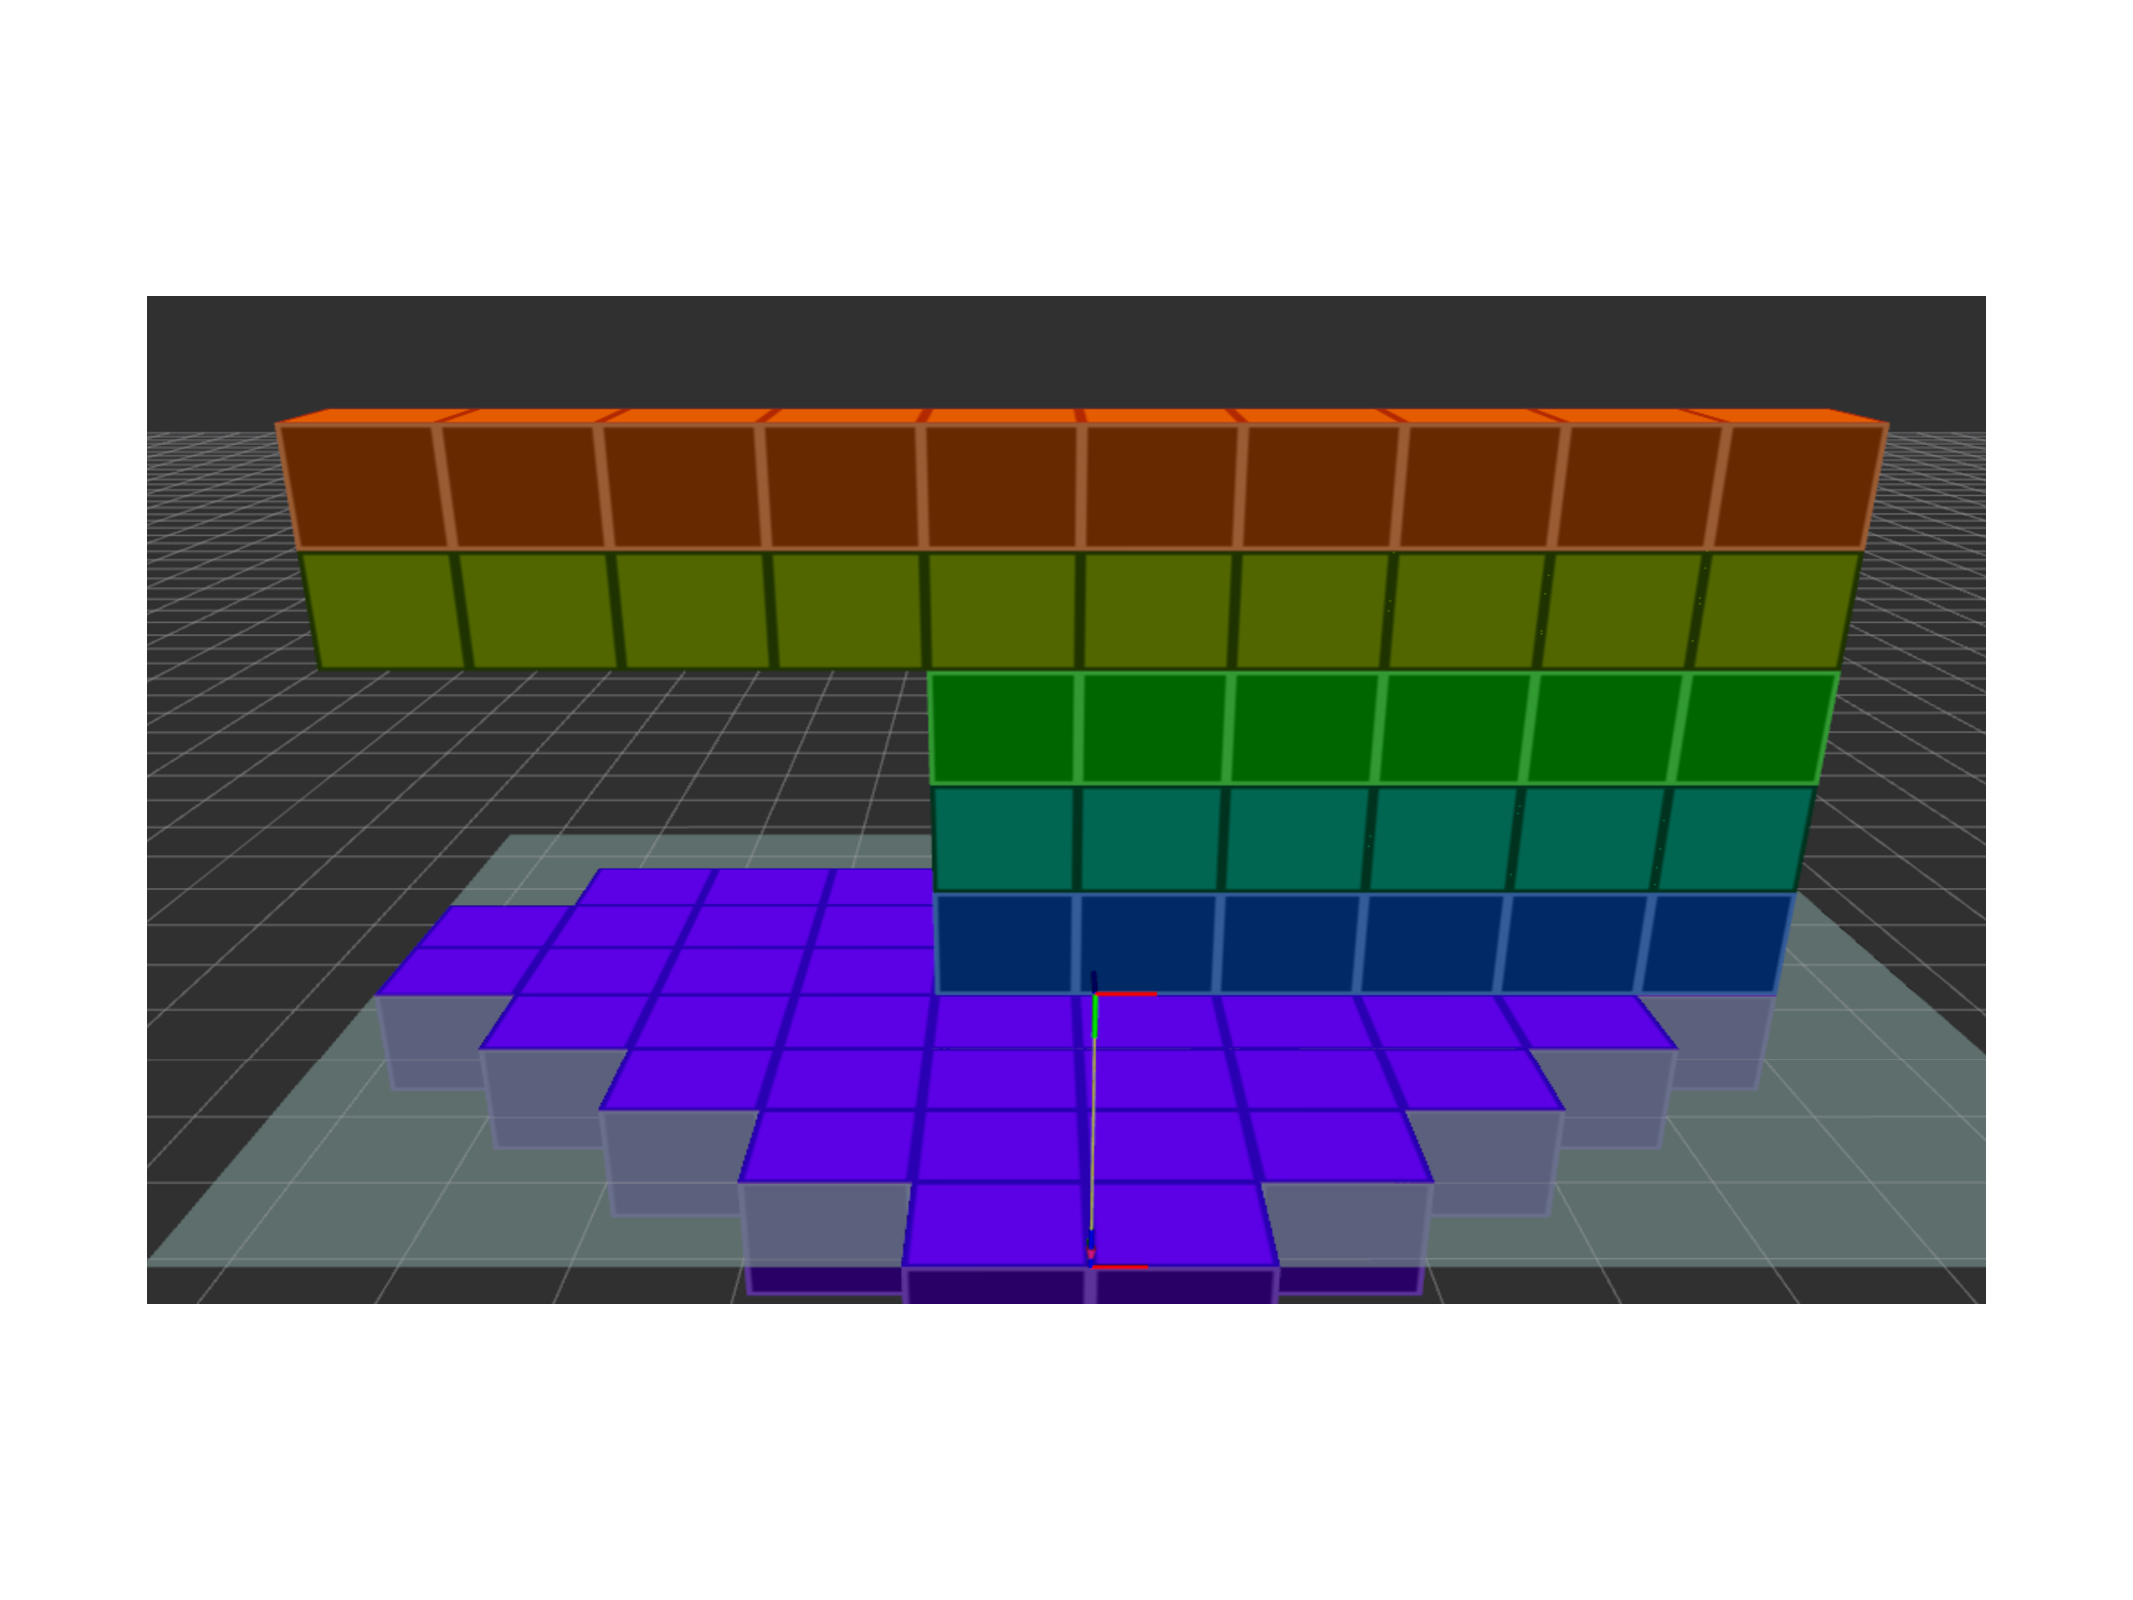
\includegraphics[height=1.4in]{figs/garage_rviz_1}%
        \vspace{-20pt}
        \caption{Resolution of 0.80 \emph{(m)}.}%
        \label{fig:game:rviz_1}
    \end{subfigure}
    \hfill\\[15pt]
   \vspace{-25pt}
   \caption{For the environment in \emph{(a)}, OctoMap's resolution impact on the drone's perception of its environment is shown in \emph{(b)}, \emph{(c)}, \emph{(d)}.}
    \label{fig:octomap_perception}
\end{figure*}

\begin{figure}[t]
\vspace{0pt}
\centering
\includegraphics[trim=0 0 30 0, clip, width=\columnwidth]
%\includegraphics[trim=0 0 0 0, clip, width=1.0
%\linewidth]%
{figs/octomap_resolution_case_study}
%{figs/octomap_resolution_with_boxes}
%\vspace{-50pt}
\vspace{-23pt}
\caption{Reduction in OctoMap resolution (accuracy) can be traded off with processing time. Increasing the $x$-axis means larger voxels to represent the space more coarsely (less accurately). A 6.5X reduction in resolution results in a 4.5X improvement in processing time.}
%\vspace{15pt}
\label{fig:octrest}
\end{figure}


\subsection{An Energy Case Study} 

Focusing on energy efficiency, we conduct a kernel/environment sensitivity analysis using the OctoMap node~\cite{octomap}, which is a major bottleneck in three of our end to end applications, namely package delivery, 3D mapping and search and rescue. OctoMap is used for the modeling of various environments without prior assumptions. The map of the environment is maintained in an efficient tree-like data structure while keeping track of the free, occupied and unknown areas. Both planning and collision avoidance kernels use OctoMap to make safe flight possible, via costly compute cycles, by only allowing navigation through free space. Due to its implementation efficiency, OctoMap is widely adopted in the robotics community. Its broad adoption and impact in two out of three stages (Perception and Planning) makes this kernel highly general and important for optimization.

The size of the voxels in OctoMap, i.e. the map's resolution, introduces accuracy versus flight-time/energy trade-off. By lowering the resolution, i.e. increasing \emph{voxel} sizes, obstacle boundaries get inflated, hence the drone's perception of the environment and the objects within it becomes inaccurate. We illustrate the impact of OctoMap resolution on the drone's perception using \Fig{fig:octomap_perception}. \Fig{fig:garage_sim} {shows the environment and  Figures~\ref{fig:rviz__15}, \ref{fig:game:rviz__5}, \ref{fig:game:rviz_1} show the drone's perception of the environment as a function of OctoMap resolution. When the resolution is lowered, the voxels size increases to the point that the drone fails to recognize the openings as possible passageways to plan through (Figure~\ref{fig:game:rviz_1}). This results in mission time inefficiency and failures depending on the environment.

To examine the accuracy versus performance trade off, we measured OctoMap kernel's processing time (running in isolation) while varying its resolution knob. \Fig{fig:octrest} shows that as planning resolution increases (i.e., voxels are larger so space is represented more coarsely and hence less accurately), performance improves dramatically because less compute is needed. Going from one extreme to another, when planning resolution goes from less than 0.2~m to 1.0~m ($x$-axis), OctoMap's processing time (or update rate) goes from more than 0.4~seconds to less than 0.1~seconds ($y$-axis). In other words, a 6.5X reduction in accuracy results in a 4.5X improvement in processing time.


\begin{figure}[t]
%\vspace{-5pt}
\centering
\includegraphics[trim=0 0 0 0, clip, width=\columnwidth]
%\includegraphics[trim=0 0 -5 -25, clip, width=0.9\linewidth]
%\includegraphics[height=5cm,keepaspectratio]
%\includegraphics[width=\columnwidth]%
%\includegraphics[trim={0 0 0 5cm}, clip, width=\columnwidth]%
{figs/energy-case-study}
\vspace{-23pt}
%\vspace{-15pt}
\caption{Switching between OctoMap resolutions dynamically leads to successfully finishing the mission compared to 0.80~m. It also leads to battery life improvement compared to 0.15~m. The $y$-axis in the top graph is the battery left on the drone upon mission completion.}
%\vspace{15pt}
\label{fig:dual-res}
\end{figure}



\begin{comment}
\begin{table}[t]
\vspace*{20pt}
\centering
\vspace{-14pt}
\caption{Switching between OctoMap resolutions dynamically leads to mission success compared to 0.8~m, and compared to 0.15~m we consume less energy and thus retain more battery.}
\label{tbl:octopt}
\resizebox{1.0\columnwidth}{!}{
\begin{tabular}{l|l|l|l|}
\cline{2-4}
\textbf{Resolution {(m)}}       & \textbf{Mission Status} & \textbf{Battery  (\%)} \\ \hline
\multicolumn{1}{|l|}{\multirow{3}{*}{\textbf{Package Delivery}}} & \textit{0.8}              & \cellcolor{red!25}Fail                    &   0           \\ \cline{2-4} 
\multicolumn{1}{|l|}{}                                           & \textit{0.15}             & Pass                    &    81.00          \\ \cline{2-4} 
\multicolumn{1}{|l|}{}                                           & \textit{Chameleon (0.8, 0.15)} & Pass                    &   \cellcolor{green!25}86.00           \\ \hline
\multicolumn{1}{|l|}{\multirow{3}{*}{\textbf{Mapping}}}          & \textit{0.8}              & \cellcolor{red!25}Fail                    & 0           \\ \cline{2-4} 
\multicolumn{1}{|l|}{}                                           & \textit{0.15}             & Pass                    & 39.03        \\ \cline{2-4} 
\multicolumn{1}{|l|}{}                                           & \textit{Chameleon (0.8, 0.15)} & Pass                    & \cellcolor{green!25}53.83        \\ \hline
\multicolumn{1}{|l|}{\multirow{3}{*}{\textbf{Search and Rescue}}}              & \textit{0.8}              & \cellcolor{red!25}Fail                    & 0         \\ \cline{2-4} 
\multicolumn{1}{|l|}{}                                           & \textit{0.15}             & Pass                    & 24.21        \\ \cline{2-4} 
\multicolumn{1}{|l|}{}                                           & \textit{Chameleon (0.8, 0.15)} & Pass                    & \cellcolor{green!25}57.87        \\ \hline
\end{tabular}
}
\end{table}
\end{comment}


Certain aspects like obstacle density in the environment determine the ``ideal'' OctoMap resolution. In low-density environments, where the drone has many obstacle-free paths to take, a low resolution can suffice. In dense environments, low resolutions can deprive the drone of viable obstacle-free paths because the drone perceives the obstacles to be larger than they are in the real world, and so plans to avoid them. Since the drone's environment constantly changes, a dynamic approach where a runtime sets the resolution is ideally desirable.

We study two environments during the mission, namely outdoors (low obstacle density) and indoors (high obstacle density). \Fig{fig:dual-res} shows the result of two static (predetermined) resolutions, 0.15~m and 0.80~m, and our dynamic approach that multiplexes between the two appropriately.\footnote{Resolutions are based on the environment like the door width size. A 0.15~m resolution is chosen to ensure that the drone (diagonal width of 0.65~m) considers an average door (width of 0.82~m) as an opening for planning.} The dynamic approach allows improvement of battery consumption by up to 1.8X. 
%life for up to 43\%. To compute this improvement, we calculate the difference between the dynamic and static battery consumption and divide it by the static value. For example, for SAR, $\frac{(76\%- 43\%)}{76\%}$ leads to a 43\% improvement. 
Intuitively, as compute reduces, OctoMap bottleneck eases, and therefore the drone completes its mission faster. The figure also highlights another interesting relationship that statically choosing the 0.80~m resolution to optimize for compute (only) causes the drone to fail its mission since it is unable to plan paths through narrow openings in the indoor environments. Instead, by switching between the two resolutions according to the environment's obstacle density, the dynamic approach is able to balance OctoMap computation with mission feasibility and energy, holistically. Therefore, in all cases, the dynamic approach uses less energy and retains more battery life at mission end time.


% Please add the following required packages to your document preamble:
% \usepackage{multirow}


\subsection{A Reliability Case Study}

Reliability is an especially important topic in the context of autonomous vehicles~\cite{reli-1, reli-2, reli-3, reli-4}. Traditionally, it is common to study the susceptibility of execution to errors that manifest in programs and the architecture. In autonomous vehicles, errors or ``noise'' in the data can arise from sensor inputs. 

We investigate the impact of sensor noise on the performance of our package delivery application, specifically its perception stage. The data is summarized in Table~\ref{tbl:noise-data}. We inject Gaussian noise with a range of standard deviations (0 to 1.5~m) into the depth readings of the drone's RGBD camera. The sensory noise distorts the drone's perception of the obstacles in its environment, and we found such noise \emph{inflates} obstacles, making them appear larger than they are in reality. This causes the drone to re-plan its trajectories more often, as it assumes that its planned path will collide into objects that are actually further away than they seem. The more the drone re-plans its paths, the longer it takes to reach its destination, which increases it mission time by up to 90\%. It is also important to note that when noise values reach greater than a certain value, it causes the drone to fail in its mission altogether, e.g. noise with the standard deviation of 1.5~m results the drone to fail reaching its delivery destination in 10\% of its total runs. 

In addition to injecting noise in the sensor subsystem, we can also inject errors directly into the compute subsystem to ``simulate'' soft errors and transient bit flips in logic. Such a capability can be used to conduct vulnerability analysis~\cite{mukherjee2005soft}.
